\documentclass[../relazione.tex]{subfiles}
\graphicspath{{\subfix{../images/}}}

\begin{document}
\section{Analisi delle prestazioni su diversi Device}
Riportiamo ora i tempi medi di runtime ottenuti eseguendo dei test con la versione \textit{Rectangular} su un dataset di 4096 elementi eseguito per 15 volte su ognuno dei seguenti dispositivi:
\begin{enumerate}
    \item NVIDIA CUDA GeForce GTX 1650 with Max-Q Design				
    \item Intel(R) UHD Graphics
    \item Intel(R) Core(TM) i7-10710U CPU @ 1.10GHz
\end{enumerate}

\subsection{Versione \textit{Rectangular}}
\begin{figure}[H]
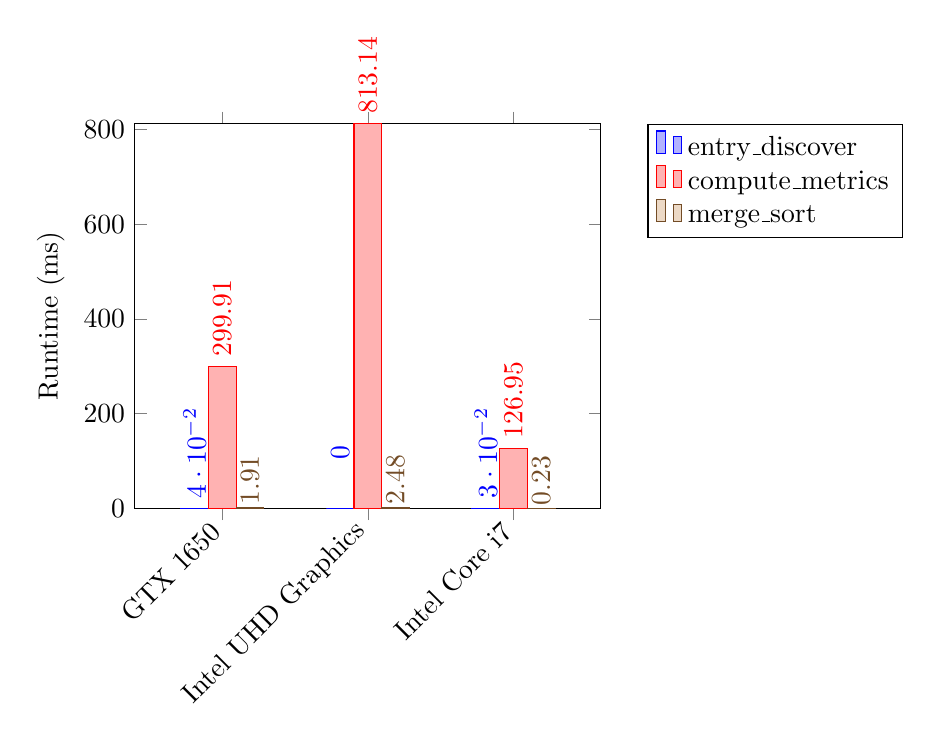
\begin{tikzpicture}
\begin{axis}[
symbolic x coords={
GTX 1650,
Intel UHD Graphics,
Intel Core i7
},
xtick=data,
x tick label style={rotate=45,anchor=east},
nodes near coords,
every node near coord/.append style={rotate=90, anchor=center},
ylabel=Runtime (ms),
legend style={at={(1.1, 0.85)}, anchor=west},
ybar=0pt,
legend cell align={left},
enlarge x limits=0.3,
enlarge y limits=0,
width=7.5cm,
]
\addplot+[every node near coord/.append style={yshift=10pt, xshift=30pt}] coordinates { %entries discover
(GTX 1650, 0.04)
(Intel UHD Graphics, 0.00)
(Intel Core i7, 0.03)
};
\addplot+[every node near coord/.append style={xshift=0pt, anchor=west}] coordinates { %compute metrics
(GTX 1650, 299.91)
(Intel UHD Graphics, 813.14)
(Intel Core i7, 126.95)
};
\addplot+[every node near coord/.append style={yshift=-10pt, xshift=0pt}] coordinates { %mergesort
(GTX 1650, 1.91)
(Intel UHD Graphics, 2.48)
(Intel Core i7, 0.23)
};
\legend{entry\_discover, compute\_metrics, merge\_sort}
\end{axis}
\end{tikzpicture}
\caption{Tempi di runtime della versione \textit{Rectangular}}
\end{figure}

\subsection{Versione \textit{Rectangular} vettorizzata}

\begin{figure}[H]
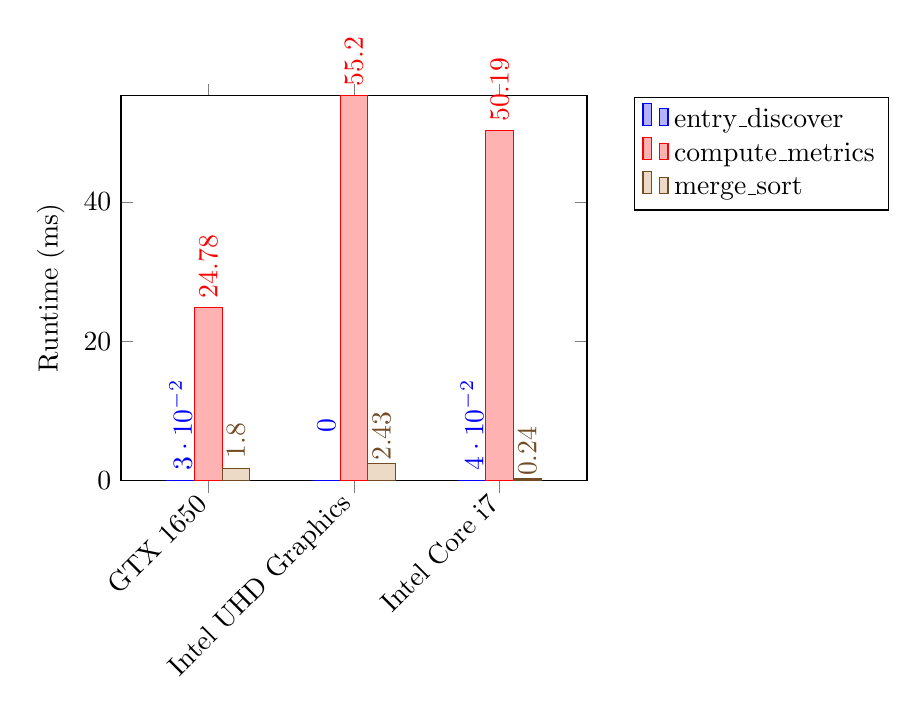
\begin{tikzpicture}
\begin{axis}[
symbolic x coords={
GTX 1650,
Intel UHD Graphics,
Intel Core i7
},
xtick=data,
x tick label style={rotate=45,anchor=east},
nodes near coords,
every node near coord/.append style={rotate=90, anchor=center},
ylabel=Runtime (ms),
legend style={at={(1.1, 0.85)}, anchor=west},
ybar=0pt,
legend cell align={left},
enlarge x limits=0.3,
enlarge y limits=0,
width=7.5cm,
]
\addplot+[every node near coord/.append style={yshift=10pt, xshift=30pt}] coordinates { %entries discover
(GTX 1650, 0.03)
(Intel UHD Graphics, 0.00)
(Intel Core i7, 0.04)
};
\addplot+[every node near coord/.append style={xshift=0pt, anchor=west}] coordinates { %compute metrics
(GTX 1650, 24.78)
(Intel UHD Graphics, 55.20)
(Intel Core i7, 50.19)
};
\addplot+[every node near coord/.append style={yshift=-10pt, xshift=0pt}] coordinates { %mergesort
(GTX 1650, 1.80)
(Intel UHD Graphics, 2.43)
(Intel Core i7, 0.24)
};
\legend{entry\_discover, compute\_metrics, merge\_sort}
\end{axis}
\end{tikzpicture}
\caption{Tempi di runtime della versione \textit{Rectangular} vettorizzata}
\end{figure}


\subsection{Andamento delle prestazioni}
Si riportano i risultati dei test eseguiti su una GPU NVIDIA GTX 1650 con dataset di varia grandezza. Per ogni dataset sono state eseguite 15 iterazioni con la versione \textit{Rectangular} vettorizzata dei kernel e successivamente sono stati calcolati i tempi medi di runtime:

\begin{center}
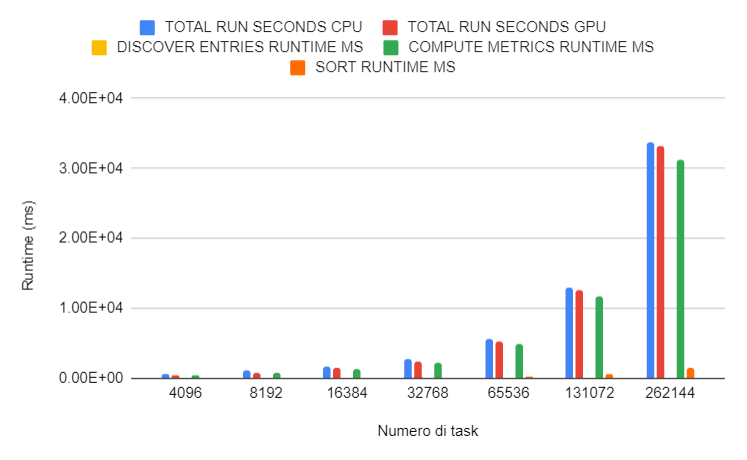
\includegraphics[scale=0.8]{images/andamento_prestazioni.png}
\end{center}

L'andamento delle prestazioni all'aumentare del numero di task è in linea con l'analisi asintotica presentata precedentemente. 

\end{document}